\documentclass[]{article}
\usepackage{lmodern}
\usepackage{amssymb,amsmath}
\usepackage{ifxetex,ifluatex}
\usepackage{fixltx2e} % provides \textsubscript
\ifnum 0\ifxetex 1\fi\ifluatex 1\fi=0 % if pdftex
  \usepackage[T1]{fontenc}
  \usepackage[utf8]{inputenc}
\else % if luatex or xelatex
  \ifxetex
    \usepackage{mathspec}
  \else
    \usepackage{fontspec}
  \fi
  \defaultfontfeatures{Ligatures=TeX,Scale=MatchLowercase}
\fi
% use upquote if available, for straight quotes in verbatim environments
\IfFileExists{upquote.sty}{\usepackage{upquote}}{}
% use microtype if available
\IfFileExists{microtype.sty}{%
\usepackage{microtype}
\UseMicrotypeSet[protrusion]{basicmath} % disable protrusion for tt fonts
}{}
\usepackage[margin=1in]{geometry}
\usepackage{hyperref}
\hypersetup{unicode=true,
            pdftitle={Supplementary for GCalignR: An R package for aligning Gas-Chromatography data},
            pdfauthor={Meinolf Ottensmann, Martin A. Stoffel, Barbara Caspers, Joseph I. Hoffman},
            pdfborder={0 0 0},
            breaklinks=true}
\urlstyle{same}  % don't use monospace font for urls
\usepackage{color}
\usepackage{fancyvrb}
\newcommand{\VerbBar}{|}
\newcommand{\VERB}{\Verb[commandchars=\\\{\}]}
\DefineVerbatimEnvironment{Highlighting}{Verbatim}{commandchars=\\\{\}}
% Add ',fontsize=\small' for more characters per line
\newenvironment{Shaded}{}{}
\newcommand{\KeywordTok}[1]{\textbf{{#1}}}
\newcommand{\DataTypeTok}[1]{\textcolor[rgb]{0.50,0.00,0.00}{{#1}}}
\newcommand{\DecValTok}[1]{\textcolor[rgb]{0.00,0.00,1.00}{{#1}}}
\newcommand{\BaseNTok}[1]{\textcolor[rgb]{0.00,0.00,1.00}{{#1}}}
\newcommand{\FloatTok}[1]{\textcolor[rgb]{0.50,0.00,0.50}{{#1}}}
\newcommand{\ConstantTok}[1]{\textcolor[rgb]{0.00,0.00,0.00}{{#1}}}
\newcommand{\CharTok}[1]{\textcolor[rgb]{1.00,0.00,1.00}{{#1}}}
\newcommand{\SpecialCharTok}[1]{\textcolor[rgb]{1.00,0.00,1.00}{{#1}}}
\newcommand{\StringTok}[1]{\textcolor[rgb]{0.87,0.00,0.00}{{#1}}}
\newcommand{\VerbatimStringTok}[1]{\textcolor[rgb]{0.87,0.00,0.00}{{#1}}}
\newcommand{\SpecialStringTok}[1]{\textcolor[rgb]{0.87,0.00,0.00}{{#1}}}
\newcommand{\ImportTok}[1]{{#1}}
\newcommand{\CommentTok}[1]{\textcolor[rgb]{0.50,0.50,0.50}{\textit{{#1}}}}
\newcommand{\DocumentationTok}[1]{\textcolor[rgb]{0.50,0.50,0.50}{\textit{{#1}}}}
\newcommand{\AnnotationTok}[1]{\textcolor[rgb]{0.50,0.50,0.50}{\textbf{\textit{{#1}}}}}
\newcommand{\CommentVarTok}[1]{\textcolor[rgb]{0.50,0.50,0.50}{\textbf{\textit{{#1}}}}}
\newcommand{\OtherTok}[1]{{#1}}
\newcommand{\FunctionTok}[1]{\textcolor[rgb]{0.00,0.00,0.50}{{#1}}}
\newcommand{\VariableTok}[1]{{#1}}
\newcommand{\ControlFlowTok}[1]{{#1}}
\newcommand{\OperatorTok}[1]{{#1}}
\newcommand{\BuiltInTok}[1]{{#1}}
\newcommand{\ExtensionTok}[1]{{#1}}
\newcommand{\PreprocessorTok}[1]{\textbf{{#1}}}
\newcommand{\AttributeTok}[1]{{#1}}
\newcommand{\RegionMarkerTok}[1]{{#1}}
\newcommand{\InformationTok}[1]{\textcolor[rgb]{0.50,0.50,0.50}{\textbf{\textit{{#1}}}}}
\newcommand{\WarningTok}[1]{\textcolor[rgb]{1.00,0.00,0.00}{\textbf{{#1}}}}
\newcommand{\AlertTok}[1]{\textcolor[rgb]{0.00,1.00,0.00}{\textbf{{#1}}}}
\newcommand{\ErrorTok}[1]{\textcolor[rgb]{1.00,0.00,0.00}{\textbf{{#1}}}}
\newcommand{\NormalTok}[1]{{#1}}
\usepackage{longtable,booktabs}
\usepackage{graphicx,grffile}
\makeatletter
\def\maxwidth{\ifdim\Gin@nat@width>\linewidth\linewidth\else\Gin@nat@width\fi}
\def\maxheight{\ifdim\Gin@nat@height>\textheight\textheight\else\Gin@nat@height\fi}
\makeatother
% Scale images if necessary, so that they will not overflow the page
% margins by default, and it is still possible to overwrite the defaults
% using explicit options in \includegraphics[width, height, ...]{}
\setkeys{Gin}{width=\maxwidth,height=\maxheight,keepaspectratio}
\IfFileExists{parskip.sty}{%
\usepackage{parskip}
}{% else
\setlength{\parindent}{0pt}
\setlength{\parskip}{6pt plus 2pt minus 1pt}
}
\setlength{\emergencystretch}{3em}  % prevent overfull lines
\providecommand{\tightlist}{%
  \setlength{\itemsep}{0pt}\setlength{\parskip}{0pt}}
\setcounter{secnumdepth}{0}
% Redefines (sub)paragraphs to behave more like sections
\ifx\paragraph\undefined\else
\let\oldparagraph\paragraph
\renewcommand{\paragraph}[1]{\oldparagraph{#1}\mbox{}}
\fi
\ifx\subparagraph\undefined\else
\let\oldsubparagraph\subparagraph
\renewcommand{\subparagraph}[1]{\oldsubparagraph{#1}\mbox{}}
\fi

%%% Use protect on footnotes to avoid problems with footnotes in titles
\let\rmarkdownfootnote\footnote%
\def\footnote{\protect\rmarkdownfootnote}

%%% Change title format to be more compact
\usepackage{titling}

% Create subtitle command for use in maketitle
\newcommand{\subtitle}[1]{
  \posttitle{
    \begin{center}\large#1\end{center}
    }
}

\setlength{\droptitle}{-2em}
  \title{Supplementary for ``GCalignR: An R package for aligning
Gas-Chromatography data''}
  \pretitle{\vspace{\droptitle}\centering\huge}
  \posttitle{\par}
  \author{Meinolf Ottensmann, Martin A. Stoffel, Barbara Caspers, Joseph I.
Hoffman}
  \preauthor{\centering\large\emph}
  \postauthor{\par}
  \predate{\centering\large\emph}
  \postdate{\par}
  \date{2016-12-01}


\begin{document}
\maketitle

\subsection{Published alignment tools for
gas-chromatography}\label{published-alignment-tools-for-gas-chromatography}

There is a small number of alignment procedures that are available to
handle gas-chromatography data \emph{without} the aid of additional
information about mass spectra which require the use of GC-MS as
analytical pathway.

\begin{longtable}[]{@{}ccccccc@{}}
\caption{Peer-reviewed alignment tools for gas-chromatography data.
Note: Unlisted are programs using mass-spectra of GC-MS
runs}\tabularnewline
\toprule
\begin{minipage}[b]{0.10\columnwidth}\centering\strut
Program\strut
\end{minipage} & \begin{minipage}[b]{0.11\columnwidth}\centering\strut
Availability\strut
\end{minipage} & \begin{minipage}[b]{0.08\columnwidth}\centering\strut
Platform\strut
\end{minipage} & \begin{minipage}[b]{0.12\columnwidth}\centering\strut
Visualisation\strut
\end{minipage} & \begin{minipage}[b]{0.22\columnwidth}\centering\strut
Limitations\strut
\end{minipage} & \begin{minipage}[b]{0.05\columnwidth}\centering\strut
Year\strut
\end{minipage} & \begin{minipage}[b]{0.14\columnwidth}\centering\strut
Source\strut
\end{minipage}\tabularnewline
\midrule
\endfirsthead
\toprule
\begin{minipage}[b]{0.10\columnwidth}\centering\strut
Program\strut
\end{minipage} & \begin{minipage}[b]{0.11\columnwidth}\centering\strut
Availability\strut
\end{minipage} & \begin{minipage}[b]{0.08\columnwidth}\centering\strut
Platform\strut
\end{minipage} & \begin{minipage}[b]{0.12\columnwidth}\centering\strut
Visualisation\strut
\end{minipage} & \begin{minipage}[b]{0.22\columnwidth}\centering\strut
Limitations\strut
\end{minipage} & \begin{minipage}[b]{0.05\columnwidth}\centering\strut
Year\strut
\end{minipage} & \begin{minipage}[b]{0.14\columnwidth}\centering\strut
Source\strut
\end{minipage}\tabularnewline
\midrule
\endhead
\begin{minipage}[t]{0.10\columnwidth}\centering\strut
GCALIGNER 1.0\strut
\end{minipage} & \begin{minipage}[t]{0.11\columnwidth}\centering\strut
freeware\strut
\end{minipage} & \begin{minipage}[t]{0.08\columnwidth}\centering\strut
Java\strut
\end{minipage} & \begin{minipage}[t]{0.12\columnwidth}\centering\strut
None\strut
\end{minipage} & \begin{minipage}[t]{0.22\columnwidth}\centering\strut
Last sample remains unaligned\strut
\end{minipage} & \begin{minipage}[t]{0.05\columnwidth}\centering\strut
2013\strut
\end{minipage} & \begin{minipage}[t]{0.14\columnwidth}\centering\strut
\{Dellicour 2013 \#8\}\strut
\end{minipage}\tabularnewline
\bottomrule
\end{longtable}

\subsection{Testing GCalignR with published
data}\label{testing-gcalignr-with-published-data}

Dellicour and Lecocq (2013) present data for three North America bumble
bee species \emph{Bombus bimaculatus}, \emph{B. ephippiatus} and
\emph{B. flavifrons}. Samples represent cephalic labial gland secretions
and are supposed to show species specific patterns. Hence, this in an
ideal data set to test both (i) the alignment efficiency of
\textbf{GCalignR} and (ii) the functionality to explore similarity
patterns by multidimensional scaling within one pipeline in \textbf{R}.

\begin{Shaded}
\begin{Highlighting}[]
\KeywordTok{library}\NormalTok{(GCalignR)}
\KeywordTok{check_input}\NormalTok{(}\DataTypeTok{data =} \StringTok{"data/d1/Table_S1_raw.txt"}\NormalTok{)}
\CommentTok{#> Warning: BEPH06 violate(s) the requirements.}
\CommentTok{#> Warning: Every sample needs to have the same number of values for each}
\CommentTok{#> variable!}
\end{Highlighting}
\end{Shaded}

Not all checks have been passed. Read warning messages and change data
accordingly

Sample \emph{BEPH06} is malformed. The last substance has not retention
time and needs to be exluded from the data set. This is an error in the
supporting information of the paper.

\begin{Shaded}
\begin{Highlighting}[]
\KeywordTok{check_input}\NormalTok{(}\DataTypeTok{data =} \StringTok{"data/d1/Table_S1_cleaned.txt"}\NormalTok{)}
\end{Highlighting}
\end{Shaded}

All checks passed! Ready for processing with align\_chromatograms

\begin{Shaded}
\begin{Highlighting}[]
\NormalTok{aligned <-}\StringTok{ }\KeywordTok{align_chromatograms}\NormalTok{(}\DataTypeTok{data =} \StringTok{"data/d1/Table_S1_raw.txt"}\NormalTok{,}
                    \DataTypeTok{conc_col_name =} \StringTok{"Area"}\NormalTok{,}
                    \DataTypeTok{max_diff_peak2mean =} \FloatTok{0.03}\NormalTok{,}
                    \DataTypeTok{min_diff_peak2peak =} \FloatTok{0.1}\NormalTok{,}
                    \DataTypeTok{rt_col_name =} \StringTok{"RT"}\NormalTok{,}
                    \DataTypeTok{delete_single_peak =} \NormalTok{F,}
                    \DataTypeTok{merge_rare_peaks =} \NormalTok{F)}
\CommentTok{#> Warning: BEPH06 violate(s) the requirements.}
\CommentTok{#> Warning: Every sample needs to have the same number of values for each}
\CommentTok{#> variable!}
\end{Highlighting}
\end{Shaded}

Not all checks have been passed. Read warning messages and change data
accordinglyRun GCalignR Start: 16:38:40

GC-data for 55 samples loaded

A reference was not specified. Hence `BBIM03' was selected on the basis
of highest average similarity to all samples (score = 18)

Start Linear Transformation with ``BBIM03'' as a reference \ldots{}Done

Start Alignment of Peaks \ldots{} This might take a while!

Do you know how well birds can see? The Northern Hawk Owl (Surnia ulula)
can detect primarily by sight a vole to eat up to a half a mile away.

Iteration 1 out of 1 \ldots{}

Merged Redundant Peaks

Peak Alignment Done

Alignment was Successful! Time: 16:41:11

\begin{Shaded}
\begin{Highlighting}[]
\KeywordTok{save}\NormalTok{(aligned, }\DataTypeTok{file =} \StringTok{"data/d1/Table_S1_aligned.RData"}\NormalTok{)}
\end{Highlighting}
\end{Shaded}

\begin{Shaded}
\begin{Highlighting}[]
\CommentTok{# aligned data}
\KeywordTok{load}\NormalTok{(}\DataTypeTok{file =} \StringTok{"data/d1/Table_S1_aligned.RData"}\NormalTok{)}
\CommentTok{# factors}
\NormalTok{factors <-}\StringTok{ }\KeywordTok{read.csv}\NormalTok{(}\StringTok{"data/d1/Table_S1_factors.csv"}\NormalTok{,}\DataTypeTok{sep =} \StringTok{";"}\NormalTok{)}
\KeywordTok{row.names}\NormalTok{(factors) <-}\StringTok{ }\NormalTok{factors[[}\StringTok{"ID"}\NormalTok{]]}
\end{Highlighting}
\end{Shaded}

Dellicour and Lecocq (2013) validated the alignment of their tool by
GC-MS. For \emph{B. flavifrons} they report a low error rate of 0.3 \%.
Hence, this data set is a good source to explore acceptable variation
among retention times that are mapped to the same substance.

\begin{Shaded}
\begin{Highlighting}[]
\NormalTok{t2 <-}\StringTok{ }\KeywordTok{read.csv}\NormalTok{(}\StringTok{"data/d1/Table_S2_modified.txt"}\NormalTok{, }\DataTypeTok{skip =} \DecValTok{1}\NormalTok{, }\DataTypeTok{sep =} \StringTok{"}\CharTok{\textbackslash{}t}\StringTok{"}\NormalTok{, }\DataTypeTok{header =} \OtherTok{FALSE}\NormalTok{)}
\CommentTok{# get the retention times}
\NormalTok{t2 <-}\StringTok{ }\NormalTok{t2[}\DecValTok{3}\NormalTok{:}\DecValTok{61}\NormalTok{,}\KeywordTok{seq}\NormalTok{(}\DecValTok{1}\NormalTok{,}\DecValTok{31}\NormalTok{,}\DecValTok{3}\NormalTok{)]}
\NormalTok{t2 <-}\StringTok{ }\KeywordTok{apply}\NormalTok{(t2, }\DataTypeTok{MARGIN =} \DecValTok{2}\NormalTok{, as.numeric)}
\NormalTok{t2 <-}\StringTok{ }\KeywordTok{data.frame}\NormalTok{(}\DataTypeTok{rt =} \KeywordTok{rowMeans}\NormalTok{(t2, }\DataTypeTok{na.rm =} \NormalTok{T), }\DataTypeTok{var =} \KeywordTok{apply}\NormalTok{(t2, }\DecValTok{1}\NormalTok{, var, }\DataTypeTok{na.rm =} \NormalTok{T), }\DataTypeTok{range =} \KeywordTok{apply}\NormalTok{(t2,}\DecValTok{1}\NormalTok{, function(x) }\KeywordTok{max}\NormalTok{(x) -}\StringTok{ }\KeywordTok{min}\NormalTok{(x))) }
\end{Highlighting}
\end{Shaded}

\subsection{NMDS}\label{nmds}

\begin{Shaded}
\begin{Highlighting}[]
\NormalTok{scent <-}\StringTok{ }\KeywordTok{norm_peaks}\NormalTok{(aligned,}\DataTypeTok{conc_col_name =} \StringTok{"Area"}\NormalTok{,}\DataTypeTok{rt_col_name =} \StringTok{"RT"}\NormalTok{,}\DataTypeTok{out =} \StringTok{"data.frame"}\NormalTok{)}
\NormalTok{scent <-}\StringTok{ }\KeywordTok{log}\NormalTok{(scent +}\StringTok{ }\DecValTok{1}\NormalTok{) }
\KeywordTok{library}\NormalTok{(vegan)}
\CommentTok{#> Loading required package: permute}
\CommentTok{#> Loading required package: lattice}
\CommentTok{#> This is vegan 2.4-1}
\NormalTok{scent <-}\StringTok{ }\NormalTok{scent[}\KeywordTok{match}\NormalTok{(}\KeywordTok{row.names}\NormalTok{(factors),}\KeywordTok{row.names}\NormalTok{(scent)),] }
\NormalTok{scent_nmds <-}\StringTok{ }\NormalTok{vegan::}\KeywordTok{metaMDS}\NormalTok{(}\DataTypeTok{comm =} \NormalTok{scent) }
\CommentTok{#> Run 0 stress 0.1556261 }
\CommentTok{#> Run 1 stress 0.1427999 }
\CommentTok{#> ... New best solution}
\CommentTok{#> ... Procrustes: rmse 0.05323072  max resid 0.2428411 }
\CommentTok{#> Run 2 stress 0.1429259 }
\CommentTok{#> ... Procrustes: rmse 0.01092181  max resid 0.07636847 }
\CommentTok{#> Run 3 stress 0.1427999 }
\CommentTok{#> ... Procrustes: rmse 2.834907e-05  max resid 0.0001252045 }
\CommentTok{#> ... Similar to previous best}
\CommentTok{#> Run 4 stress 0.1556259 }
\CommentTok{#> Run 5 stress 0.2688805 }
\CommentTok{#> Run 6 stress 0.1556259 }
\CommentTok{#> Run 7 stress 0.1519242 }
\CommentTok{#> Run 8 stress 0.2483444 }
\CommentTok{#> Run 9 stress 0.2479965 }
\CommentTok{#> Run 10 stress 0.232269 }
\CommentTok{#> Run 11 stress 0.2653986 }
\CommentTok{#> Run 12 stress 0.2667564 }
\CommentTok{#> Run 13 stress 0.1556266 }
\CommentTok{#> Run 14 stress 0.1447737 }
\CommentTok{#> Run 15 stress 0.1519241 }
\CommentTok{#> Run 16 stress 0.2349557 }
\CommentTok{#> Run 17 stress 0.1556259 }
\CommentTok{#> Run 18 stress 0.1445487 }
\CommentTok{#> Run 19 stress 0.1523269 }
\CommentTok{#> Run 20 stress 0.2339989 }
\CommentTok{#> *** Solution reached}
\NormalTok{scent_nmds <-}\StringTok{ }\KeywordTok{as.data.frame}\NormalTok{(scent_nmds$points) }
\NormalTok{scent_nmds <-}\StringTok{ }\KeywordTok{cbind}\NormalTok{(scent_nmds,}\DataTypeTok{Species =} \NormalTok{factors[[}\StringTok{"Species"}\NormalTok{]])  }
\NormalTok{ggplot2::}\KeywordTok{ggplot}\NormalTok{(}\DataTypeTok{data =} \NormalTok{scent_nmds,ggplot2::}\KeywordTok{aes}\NormalTok{(MDS1,MDS2,}\DataTypeTok{color =} \NormalTok{Species)) +}
\StringTok{    }\NormalTok{ggplot2::}\KeywordTok{geom_point}\NormalTok{(}\DataTypeTok{size =} \DecValTok{4}\NormalTok{) +}\StringTok{ }\NormalTok{ggplot2::}\KeywordTok{stat_ellipse}\NormalTok{(}\DataTypeTok{size =} \DecValTok{2}\NormalTok{) +}\StringTok{ }\NormalTok{ggplot2::}\KeywordTok{labs}\NormalTok{(}\DataTypeTok{title =} \StringTok{""}\NormalTok{, }\DataTypeTok{x =} \StringTok{"MDS1"}\NormalTok{, }\DataTypeTok{y =} \StringTok{"MDS2"}\NormalTok{) +}\StringTok{ }\NormalTok{ggplot2::}\KeywordTok{theme_void}\NormalTok{()}
\end{Highlighting}
\end{Shaded}

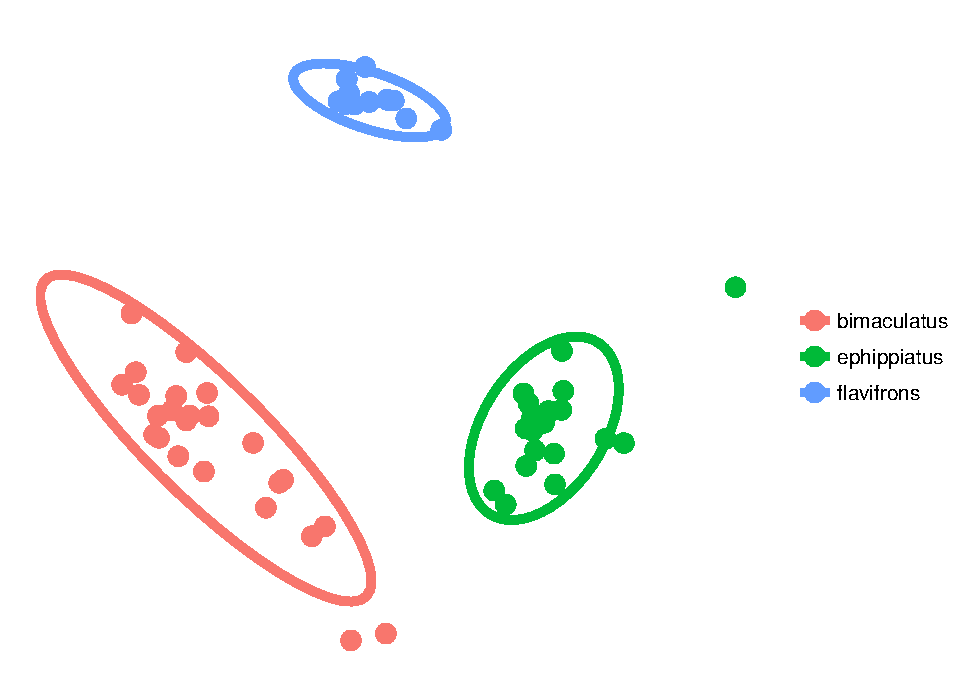
\includegraphics{Supplementary_1_files/figure-latex/unnamed-chunk-8-1.pdf}

\subsection*{References}\label{references}
\addcontentsline{toc}{subsection}{References}

\hypertarget{refs}{}
\hypertarget{ref-Dellicour.2013}{}
Dellicour, Simon, and Thomas Lecocq. 2013. ``GCALIGNER 1.0: An Alignment
Program to Compute a Multiple Sample Comparison Data Matrix from Large
Eco-Chemical Datasets Obtained by Gc.'' \emph{Journal of Separation
Science} 36 (19): 3206--9.
doi:\href{https://doi.org/10.1002/jssc.201300388}{10.1002/jssc.201300388}.


\end{document}
